\documentclass[screen, aspectratio=43]{beamer}
\usetheme[style=ntnu,language=en]{ntnu2017}
\usepackage[T1]{fontenc}
\usepackage[utf8]{inputenc}

\usepackage[english]{babel}
\usepackage{mystyle}

%\date{} % To have an empty date
\AtBeginSection[]
{
	\begin{frame}
		\frametitle{Outline}
		\tableofcontents[currentsection]
	\end{frame}
}

\begin{document}

\title{Digital datadriven model learning for online testing of hydro power plants}
\author{Sigurd Hofsmo Jakobsen}
\institute[NTNU]{Department of electrical engineering}
\date{\today}

\begin{frame}
  \titlepage
\end{frame}

\thispagestyle{empty}
\makeatletter
\def\cleartextposbox{\global\setbox\TP@holdbox\vbox{}}
\makeatother
\null\newpage\cleartextposbox
\section{Problem}
\begin{frame}
	\frametitle{Load and production balancing}
	\begin{columns}
		\begin{column}{0.5\textwidth}
				\begin{itemize}
				\item<1-> The power system frequency measures the power balance.
				\item<2-> It is the responsibility of Statnett to control the frequency.
				\item<3-> However, it is the power plant owners who can control the frequency.
			\end{itemize}
		\end{column}
		\begin{column}{0.5\textwidth}
			\begin{figure}
				\includegraphics<1>[width=0.8\textwidth]{./pictures/balance.png}
				\includegraphics<2>[width=0.8\textwidth]{./pictures/balance_statnett.png}
				\includegraphics<3->[width=0.8\textwidth]{./pictures/balance_producers.png}
			\end{figure}
		\end{column}
	\end{columns}
\end{frame}
\begin{frame}
\frametitle{Buying frequency control}
\begin{columns}
\begin{column}{0.5\textwidth}
		\begin{itemize}
		\item<1-> Statnett pays all power plant owners to provide frequency control.
		\item<2-> However, they don't provide the same quality of service.
		\item<3-> Renewable energy sources such as wind and solar don't contribute.

	\end{itemize}
\end{column}
\begin{column}{0.5\textwidth}
	\begin{figure}
		\includegraphics<1>[width=0.8\textwidth]{./pictures/fcp_response_one.tikz}
		\includegraphics<2>[width=0.8\textwidth]{./pictures/fcp_response.tikz}
		\includegraphics<3->[width=0.8\textwidth]{./pictures/res_response.tikz}
		\caption{Frequency control response to step change in frequency}
	\end{figure}
\end{column}
\end{columns}
\end{frame}
\begin{frame}
\frametitle{Future of frequency control}
\begin{columns}
\begin{column}{0.4\textwidth}
		\begin{itemize}
		\item Power plants have to pass tests to get paid to provide frequency control.
		\item Only those who pass the tests get paid for the service.
	\end{itemize}
\end{column}
\begin{column}{0.6\textwidth}
	\begin{figure}
		\includegraphics{./pictures/block.tikz}
		\caption{Test of power plant}
	\end{figure}
\end{column}
\end{columns}
\end{frame}
\begin{frame}
		\frametitle{Tests proposed by the industry}
		\begin{figure}
				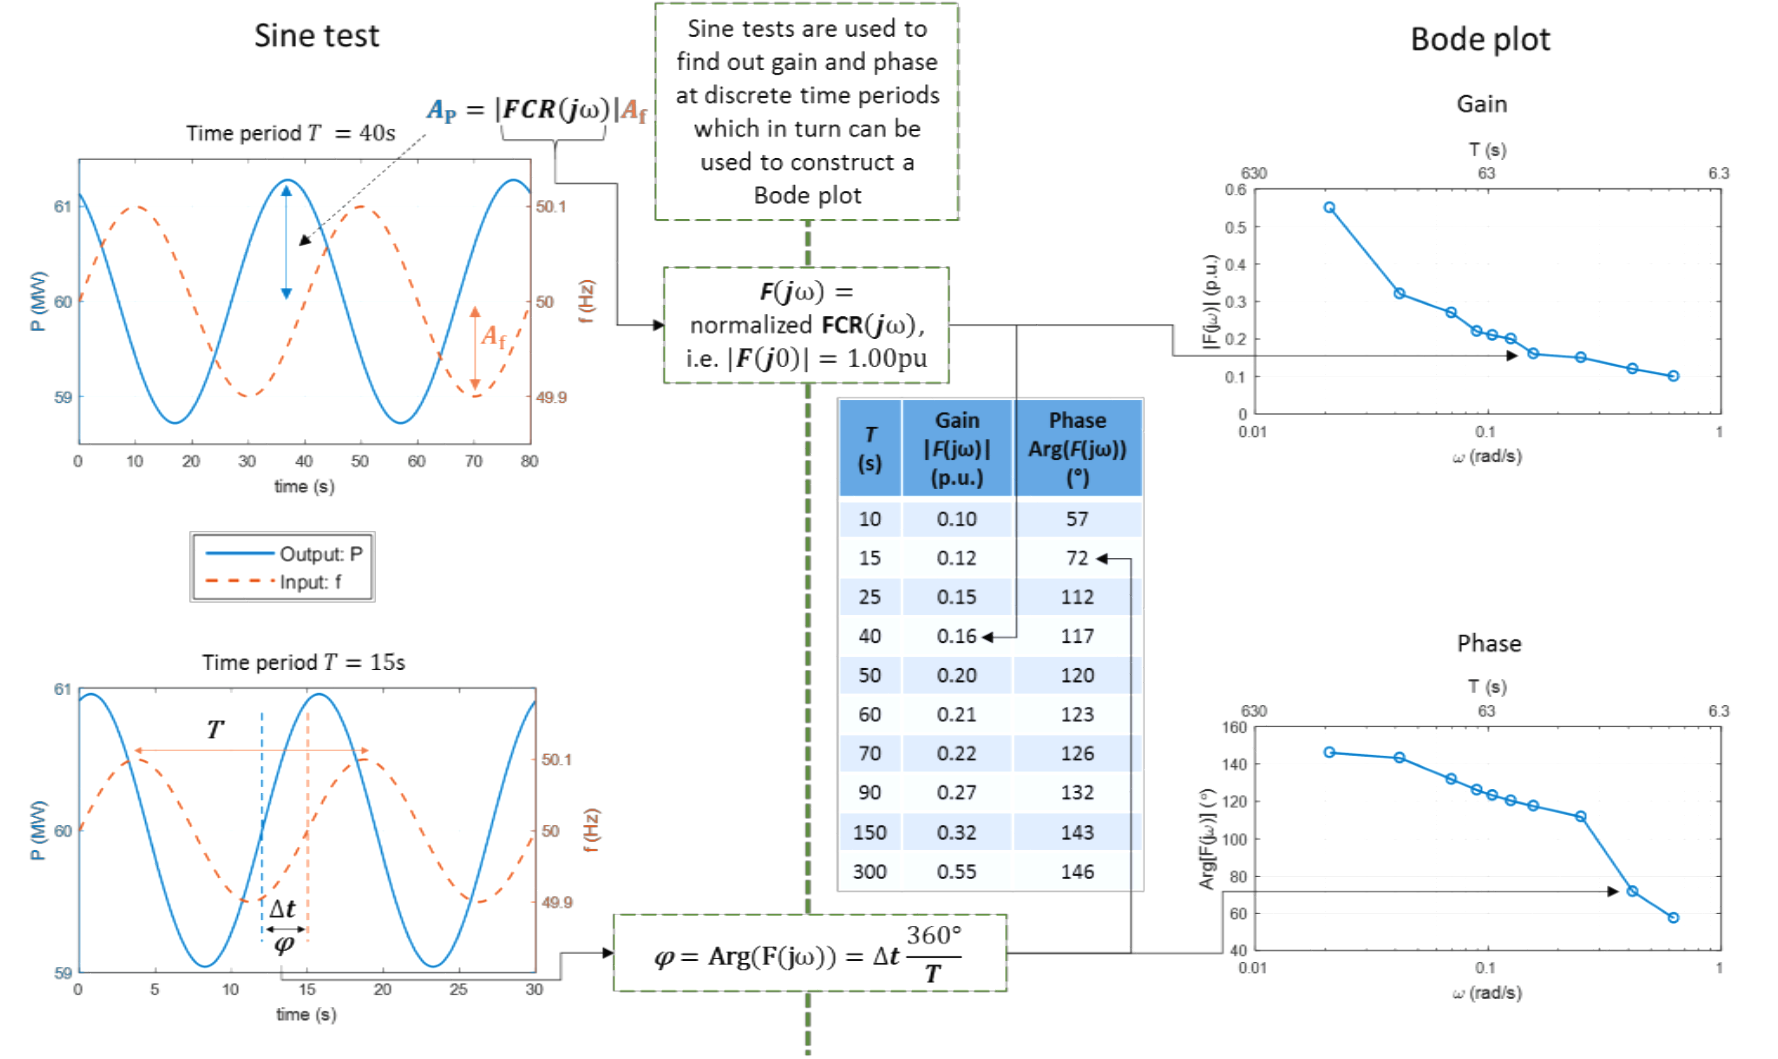
\includegraphics[width=\textwidth]{./pictures/tests.png}
				\caption{Testing procedure [source:ENTSO-E]}
		\end{figure}
\end{frame}
\begin{frame}
		\frametitle{Example from real tests}
		\begin{columns}
				\begin{column}{0.5\textwidth}
						\begin{itemize}
								\item<1-> The power plant needs to be disconnected
								\item<1-> Takes up to 20 hours.
								\item<2-> Only one sine test needed with model learning.
						\end{itemize}
			\end{column}
			\begin{column}{0.5\textwidth}
						\begin{figure}
						\includegraphics<1->[width=\textwidth]{./pictures/aura_signals.tikz}
				\end{figure}
						\includegraphics<1>[width=\textwidth]{./pictures/frd.tikz}
						\includegraphics<2>[width=\textwidth]{./pictures/frd_vs_bj.tikz}
				\end{column}
		\end{columns}
\end{frame}

\section{Paper I}
\begin{frame}
	\frametitle{Background}
	\begin{columns}
		\begin{column}{0.4\textwidth}
			\begin{itemize}
					\item<1->  Idea from\footnotemark[1] can the power plant dynamics be identified using PMUs
					\item<2-> Uses the same input and output measurements as in the requirements:
					\begin{itemize}
							\item Input: Power system frequency.
							\item Output: Electric power.
					\end{itemize}
			\end{itemize}
	\end{column}
	\begin{column}{0.6\textwidth}
			\begin{figure}
					\includegraphics<1>{./pictures/genTrafo.tikz}
					\includegraphics<2>{./pictures/block.tikz}
			\end{figure}
	\end{column}
	\end{columns}
	\footnotetext[1]{\fullcite{dinh_thuc_duong_estimation_2016}}
\end{frame}
\begin{frame}
	\frametitle{Methodology}
	\begin{columns}
			\begin{column}{0.4\textwidth}
			\begin{itemize}
					\item Collect several datasets from PMUs.
					\item Calculate power and frequency from the measurements.
					\item Identify dynamics using vector fitting.
					\item Compare models.
			\end{itemize}
			\end{column}
			\begin{column}{0.6\textwidth}
					\begin{figure}
					\includegraphics{./pictures/genTrafo.tikz}
					\end{figure}
			\end{column}
	\end{columns}
\end{frame}
\begin{frame}
	\frametitle{Vector fitting basics}
	\begin{columns}[c]
		\begin{column}{0.4\textwidth}
			\begin{itemize}
				\item<1-> Vector fitting fits a transfer function to measured input and output data
				\item<2-> It assumes the system to have the following structure.
				\item<3-> In time domain it is.
			\end{itemize}
		\end{column}
		\begin{column}{0.6\textwidth}
			\begin{itemize}
				\item[]<1->
				\begin{equation}
					Y(s) = H(s)\cdot U(s)
				\end{equation}
				\item[]<2->
				\begin{equation}
					H(s) = d + \sum^{n_p}_{i=1}\frac{r_i}{s-p_i}
				\end{equation}
				\item[]<3->
				\begin{equation}\label{eq:VFTD}
    			y(t) \approx \tilde{d} x(t) + \sum^{n_p}_{i=1} \tilde{r}_ix_i-\sum^{n_p}_{i=1}\tilde{k}_iy_i
					\end{equation}
					\begin{equation}
    \label{eq:XVFWave}
    x_i = \int^t_0 e^{\tilde{p}_i(t-\tau)}x_i(\tau)d\tau
\end{equation}
\begin{equation}
    \label{eq:YVFWave}
    y_i = \int^t_0 e^{\tilde{p}_{i}(t-\tau)}y_i(\tau)d\tau
\end{equation}
			\end{itemize}
	\end{column}
	\end{columns}
	\end{frame}

	\begin{frame}
		\frametitle{Vector fitting basics ctd.}
		\begin{itemize}
				\item Find $\tilde{d}$, $\tilde{r}_i$ and $\tilde{k}_i$ to minimize:
				\end{itemize}
				\begin{equation}
						y(t) - (\tilde{d} x(t) + \sum^{n_p}_{i=1} \tilde{r}_ix_i-\sum^{n_p}_{i=1}\tilde{k}_iy_i)
					\end{equation}

\end{frame}
		\begin{frame}[fragile]
	\frametitle{Cross validation using distant data sets}
		\includegraphics<1>[width=0.45\textwidth]{./pictures/frequencies.tikz}
		\includegraphics<1>[width=0.45\textwidth]{./pictures/powers.tikz}
		\includegraphics<2>[width=\textwidth]{./pictures/cross_val}
\end{frame}
\begin{frame}
	\frametitle{Estimated droop and bandwidth}
	\begin{figure}
		\includegraphics[width=0.6\textwidth]{./pictures/bode.tikz}
\end{figure}

		\begin{tabular}{|c|c|c|}
				\hline
				Dataset & Droop[\%] & Bandwidth[mHz] \\ \hline
				Fall 2015 & 10 & $4.16$\\ \hline
				Spring 2016 & 8 & $2.41$\\ \hline
\end{tabular}
\end{frame}
\begin{frame}
		\frametitle{Shortcoming with the paper}
		\begin{columns}
				\begin{column}{0.4\textwidth}
						\begin{itemize}
								\item No theoretical validation of the results.
								\item No simulation validation of the results.
						\end{itemize}
				\end{column}
				\begin{column}{0.6\textwidth}
						\begin{figure}
								\includegraphics{./pictures/sys.tikz}
						\end{figure}
				\end{column}
		\end{columns}
\end{frame}
\begin{frame}
		\frametitle{Main contributions to the research questions}
		\begin{columns}
				\begin{column}{0.4\textwidth}
						\begin{itemize}
								\item<1-> Promising results for 19 datasets.
								\item<2-> Developed code for interfacing with the PMU data.
						\end{itemize}
				\end{column}
				\begin{column}{0.6\textwidth}
						\begin{figure}
								\includegraphics<1>{./pictures/genTrafo.tikz}
						\end{figure}
				\end{column}
		\end{columns}
\end{frame}
		
		

		


\section{Paper II}
\begin{frame}
		\frametitle{Motivation}
		\begin{columns}
				\begin{column}{0.4\textwidth}
						\begin{itemize}
								\item Explain the problem to my co-supervisor.
								\item Create a model for analysing the identifiability of hydro power plant dynamics.
						\end{itemize}
				\end{column}
				\begin{column}{0.6\textwidth}
						\begin{figure}
								\includegraphics{./pictures/sys.tikz}
						\end{figure}
				\end{column}
		\end{columns}
\end{frame}
\begin{frame}
		\frametitle{What do we need to model?}
		\begin{columns}
				\begin{column}{0.4\textwidth}
						\begin{itemize}
							\item<1-> From the PMU we get
									\begin{itemize}
											\item<2-> Power: $\Delta P_{e1}(s)$.
											\item<3-> Frequency: $\Delta f(s)$.
									\end{itemize}
							\item<4-> We need to model how $\Delta P_{e1}(s)$ and $\Delta f(s)$ is related through the power system.
					\end{itemize}
			\end{column}
			\begin{column}{0.6\textwidth}
					\begin{figure}
					\includegraphics<1>{./pictures/genTrafo.tikz}
					\includegraphics<2->{./pictures/sys.tikz}
			\end{figure}
	\end{column}
	\end{columns}
			\end{frame}
\begin{frame}
	\frametitle{Idea behind the test system}
	\begin{columns}
		\begin{column}{0.5\textwidth}
			\begin{itemize}
				\item<1-> The frequency and power system angle is related.
				\item<2-> The angle and power is related.
				\item<3-> On matrix form.
			\end{itemize}
		\end{column}
		\begin{column}{0.5\textwidth}
			\begin{itemize}
				\item[]<1->
					\begin{equation}
							\Delta \theta(s) = \frac{2\pi f_s}{s}f(s)
						\end{equation}
				\item[]<2->
					\begin{equation}
						P_k \approx \sum_{m\in \Omega_k}{x^{-1}_{km}\theta_{km}}
					\end{equation}
				\item[]<3->
					\begin{equation}
						\mathbf{P}=\mathbf{Y}\mathbf{\theta}
					\end{equation}
			\end{itemize}
		\end{column}
	\end{columns}
\end{frame}



\section{Theoretical validation Paper III}
\begin{frame}
		\frametitle{Background}
	\begin{columns}
		\begin{column}{0.5\textwidth}
			\begin{itemize}
				\item<1-> Why do we get different results?
				\item<2-> The signals we use are corrupted by noise.
				\item<3-> Before we can talk about the different results, we need to validate our approach.
			\end{itemize}
		\end{column}
		\begin{column}{0.5\textwidth}
				\begin{figure}
					\includegraphics<1>[width=0.7\textwidth]{./pictures/bode.tikz}
					\includegraphics<2>{./pictures/v_block.tikz}
					\includegraphics<3>{./pictures/identifiability.tikz}
				\end{figure}
		\end{column}
	\end{columns}
\end{frame}
\begin{frame}
	\frametitle{System identification basic}
	\begin{columns}
		\begin{column}{0.5\textwidth}
			\begin{itemize}
				\item Assume that a data set $Z^N = \{u[n],y[n]|n=1\ldots N\}$ has been collected.
				\item The dataset $Z^N$ is assumed generated by
					\begin{equation}
						\mathcal{S}: y[n] = G_1(z,\theta_1)u[n] + H_1(z,\theta_1)e[n]
					\end{equation}
				\item Using the data set $Z^N$ we want to find the parameter vector $\theta^N$ minimizing
\begin{equation}\label{eq:pred}
		\hat{\theta}_N = \argmin_{\theta} \frac{1}{N}\sum_{n=1}^N[ H_1^{-1}(z,\theta)(y[n]-G_1(z,\theta)u[n])]^2
\end{equation}
			\end{itemize}
		\end{column}
		\begin{column}{0.5\textwidth}
			\begin{figure}
				\includegraphics{./pictures/v_block.tikz}
			\end{figure}
		\end{column}
	\end{columns}
\end{frame}
\begin{frame}
	\frametitle{Modeling used for the validation}
	\begin{columns}
		\begin{column}{0.3\textwidth}
			\begin{itemize}[<+->]
				\item The system we are identifying
					\begin{itemize}
						\item Not $G_p(s)$.
						\item Opposite $u$ and $y$ from Paper I.
					\end{itemize}
				\item We use a small power system
				\item We use a dc power flow 
				\item This results in the following block diagram
			\end{itemize}
		\end{column}
		\begin{column}{0.7\textwidth}
				\begin{equation}\only<1>{G_1(s) = \frac{G_p(s)}{1+G_p(s)G_J(s)}}\end{equation}
				\includegraphics<1>{./pictures/sys.tikz}
				\includegraphics<2>[width=0.8\textwidth]{./pictures/sld.tikz}
				\includegraphics<3>{./pictures/DC.tikz}
				\includegraphics<4>{./pictures/block_test_sys.tikz}
		\end{column}
	\end{columns}
\end{frame}
\begin{frame}
	\frametitle{Results from the theoretical validation}
	\begin{itemize}
		\item<1-> A consistent estimate of the closed loop transfer function of the turbine and electromechanical dynamics can be obtained by using:
			\begin{itemize}
				\item<2-> Measured PMU frequency as the output $u[n]$
				\item<3-> Measured PMU power as the input $y[n]$
			\end{itemize}
		\item<4-> The proof was done with the following assumptions.
			\begin{itemize}
				\item The system is excited by a load acting as a filtered white noise process
				\item The measurement error of the electrical power is negligible.
				\item The measured frequency is a good estimate of the generator speed.
			\end{itemize}
	\end{itemize}
\end{frame}
\begin{frame}
	\frametitle{Model obtained using PMU data}
	\begin{figure}
		\includegraphics[width=0.8\textwidth]{./pictures/PMU_bode.tikz}
	\end{figure}
\end{frame}
\begin{frame}
	\frametitle{Whiteness test on model identified using PMU data}
	\begin{figure}
		\includegraphics[width=0.7\textwidth]{./pictures/PMU_resid.tikz}
	\end{figure}
\end{frame}
\begin{frame}
	\frametitle{Main contributions}
	\begin{itemize}
		\item To show that the transfer function one is identifying using PMUs is $G_1(s)$.
		\item To prove under which conditions a consistent estimate of $G_1(s)$ is possible.
		\item To demonstrate the theory for identification of $G_1(s)$ on real datasets.
	\end{itemize}
\end{frame}

\section{Tests at Statkraft's power plants Paper IV}
\begin{frame}
	\frametitle{Motivation}
	\begin{itemize}
		\item Relate the results from Paper III and the new requirements.
		\item Test the methods on more real datasets.
		\item Demonstrate that industry proposed tests can be done easier.
		\item Less theoretical presentation in a more industry focused conference.
	\end{itemize}
\end{frame}
\begin{frame}
	\frametitle{Alternative requirements}
	\begin{columns}
		\begin{column}{0.5\textwidth}
				\begin{itemize}[<+->]
				\item Place requirements directly on one power plant.
				\includegraphics<1>{./pictures/sys.tikz}
				\includegraphics<1>{./pictures/req_sys.tikz}
				\item We already have an estimate of $G_1(s)$.
				\item We need to find $S(s)$
			\end{itemize}
		\end{column}
		\begin{column}{0.5\textwidth}
			\begin{figure}
				\includegraphics<2>[width=\textwidth]{./pictures/PMU_bode.tikz}
			\end{figure}
		\end{column}
	\end{columns}
\end{frame}
\begin{frame}
	\frametitle{Estimating $S(s)$}
	\begin{itemize}[<+->]
		\item
		\begin{equation} 
			G_1(s) = G_J(s)S(s)
		\end{equation}
		\item
		\begin{equation}
			G_J(s) = \frac{1}{2Hs+K_d}
		\end{equation}
		\item
		\begin{equation}
			2H>>K_d
		\end{equation}
		\item
		\begin{equation}
			S(s) \approx 2HsG_1(s)
		\end{equation}
		\item Need to estimate $H$
	\end{itemize}
\end{frame}
\begin{frame}
	\frametitle{Estimating $H$}
	\begin{figure}
			\includegraphics[width=0.9\textwidth]{./pictures/transf_comp.tikz}
	\end{figure}
\end{frame}
\begin{frame}
	\frametitle{Dataset from Statkraft}
	\begin{itemize}[<+->]
		\item Norway's biggest power producers.
		\item They performed the tests from the draft requirements
		\item By chance I had PMU measurements from the same plant.
		\end{itemize}
		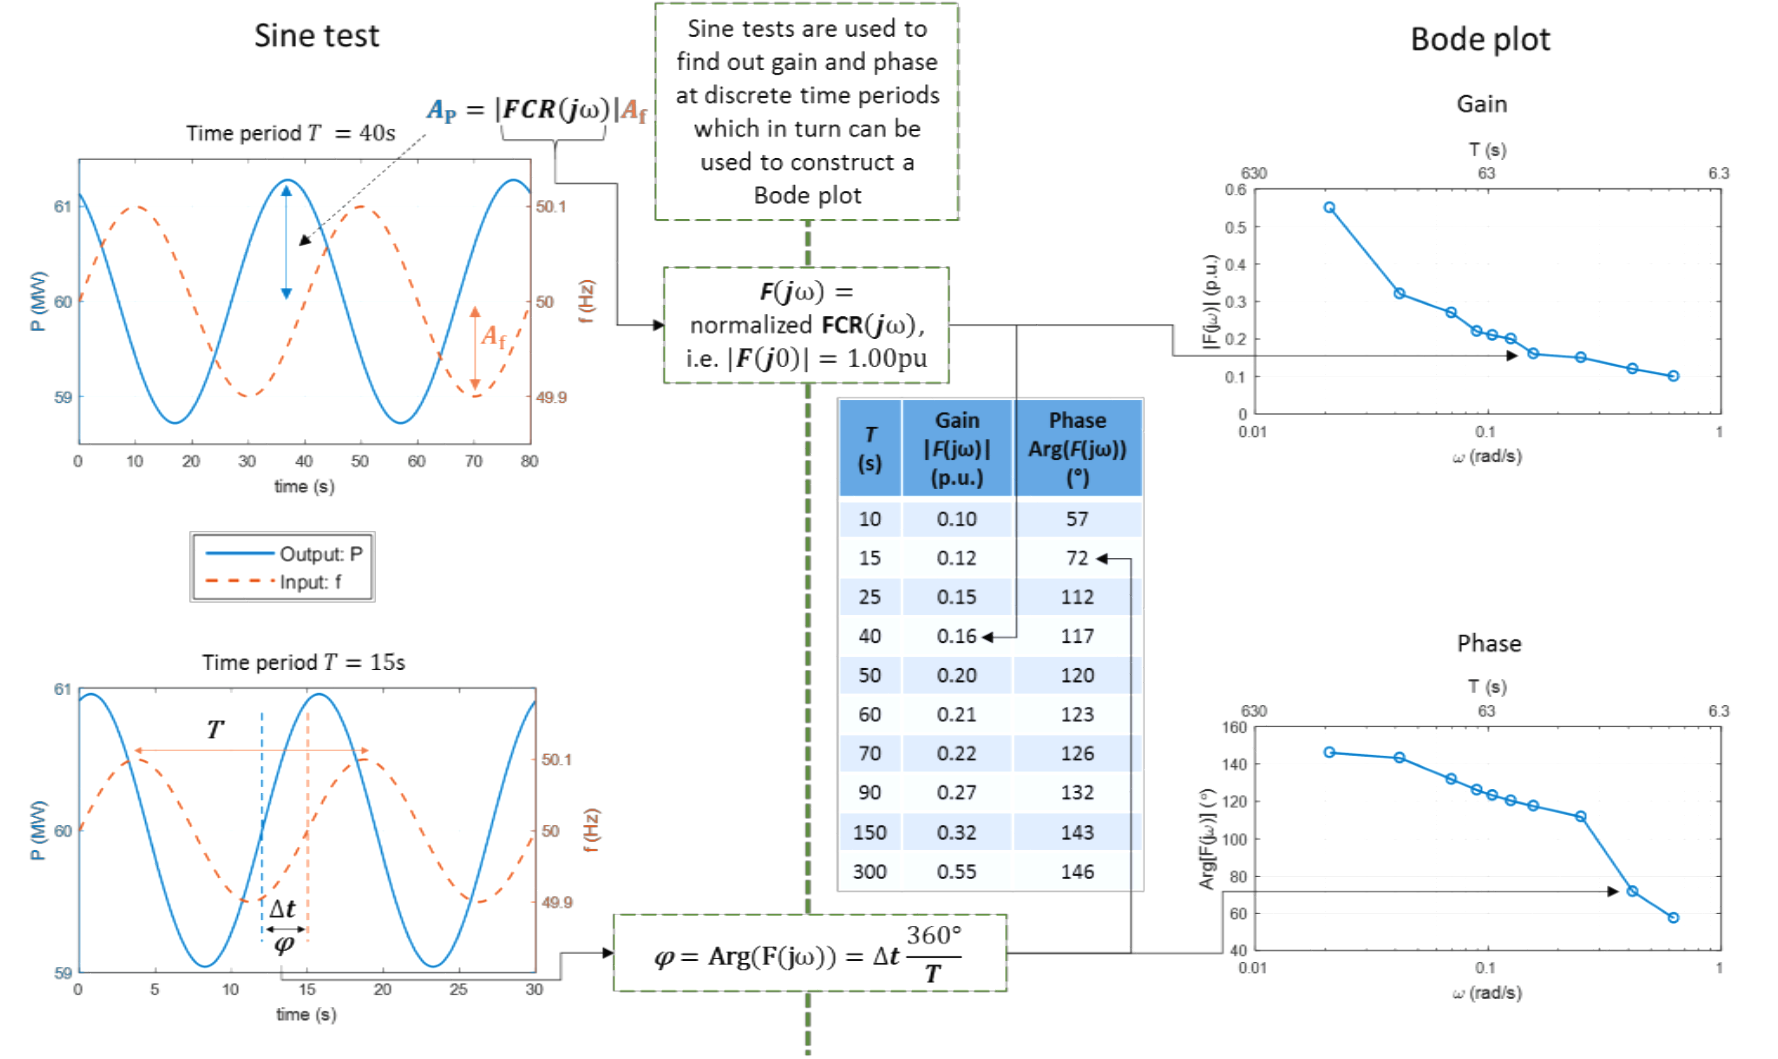
\includegraphics[width=0.8\textwidth]{./pictures/tests.png}
\end{frame}
\begin{frame}
	\frametitle{Can the industry proposed tests be done easier?}
	\begin{figure}
		\includegraphics<1->[width=0.6\textwidth]{./pictures/aura_signals.tikz}
	\end{figure}
	\begin{figure}
		\includegraphics<1>[width=0.6\textwidth]{./pictures/frd.tikz}
		\includegraphics<2>[width=0.6\textwidth]{./pictures/frd_vs_bj.tikz}
	\end{figure}
\end{frame}
\begin{frame}
	\frametitle{Datasets used}
	\begin{figure}
			\includegraphics[width=0.8\textwidth]{./pictures/signals_step.tikz}
	\end{figure}
\end{frame}
\begin{frame}
	\frametitle{Estimated sensitivity functions}
		\begin{figure}[tb]
			\includegraphics[width=0.8\textwidth]{./pictures/S_aura.tikz}
		\end{figure}
\end{frame}
\begin{frame}
	\frametitle{Estimated $G_1(s)$}
		\begin{figure}[tb]
			\includegraphics[width=0.8\textwidth]{./pictures/G1_aura.tikz}
		\end{figure}
\end{frame}
\begin{frame}
	\frametitle{Control system data in closed loop}
	\begin{figure}
		\includegraphics<1->[width=0.4\textwidth]{./pictures/Grytten_signals.tikz}
	\end{figure}
	\begin{figure}
		\includegraphics<1>[width=0.6\textwidth]{./pictures/Grytten_new_PID.tikz}
		\includegraphics<2>[width=0.6\textwidth]{./pictures/Grytten_R_5.tikz}
%		\includegraphics<3>[width=0.6\textwidth]{./pictures/Grytten_windows.tikz}
	\end{figure}
	\begin{itemize}
			\item<3>[]
			\begin{tabular}{c c c c c}
			\toprule
			Droop & $60\mathrm{min}$ & $45\mathrm{min}$ & $30\mathrm{min}$ & $15\mathrm{min}$ \\
			\midrule
			$10\%$ & $9.5\%$ & $9.5\%$ & $9.5\%$ & $9.5\%$ \\
			$6\%$ & $6.2\%$ & $6.0\%$ & $5.9\%$ & $6.1\%$ \\
			$5\%$ & $4.9\%$ & $4.9\%$ & $5.0\%$ & $5.1\%$ \\
			$3\%$ & $3.1\%$ & $3.1\%$ & $3.1\%$ & $2.9\%$ \\
			$2\%$ & $2.0\%$ & $1.8\%$ & $1.8\%$ & $1.7\%$\\
			\bottomrule
		\end{tabular}
	\end{itemize}
\end{frame}
\begin{frame}
	\frametitle{Main Contributions}
	\begin{itemize}
		\item Proposal for alternative tests.
		\item Demonstrating that the proposed methods can detect parameter changes.
		\item Demonstrated that the industry proposed tests can be done easier.
	\end{itemize}
\end{frame}

\section{An extension of Paper IV, with more discussion, simulation comparisons and more simulation validations Paper V}
\begin{frame}
	\frametitle{Motivation}
	\begin{itemize}
		\item Test with a more detailed power plant model.
		\item Test with a more detailed power system model.
		\item Investigate some of the assumptions from previous papers.
	\end{itemize}
\end{frame}
\begin{frame}
	\frametitle{More detailed power plant model}
	\begin{figure}
		\includegraphics{./pictures/PID.tikz}
	\begin{figure}
		\includegraphics{./pictures/governor.tikz}
	\end{figure}
	\end{figure}
	\begin{figure}
		\includegraphics{./pictures/turbine.tikz}
	\end{figure}
\end{frame}
\begin{frame}
	\frametitle{More detailed power system model}
	\begin{columns}
		\begin{column}{0.5\textwidth}
			\begin{itemize}
				\item<1-> Added the frequency divider formula to the simple test system.
				\item<2-> Used the Nordic 44 test system in PSS/E.
			\end{itemize}
		\end{column}
		\begin{column}{0.5\textwidth}
			\begin{itemize}
					\item<1>[]
				\begin{equation}
					\omega_l = \mathbf{1}+\mathbf{D}(\omega_e-\mathbf{1})
				\end{equation}
				where
				\begin{equation}
					\mathbf{D} = -\mathbf{B}_{22}^{-1}\mathbf{B}_{21}
				\end{equation}
			\end{itemize}
			\begin{figure}
				\includegraphics<2>[width=\textwidth]{./pictures/Nordic44-Bilde}
			\end{figure}
		\end{column}
	\end{columns}
\end{frame}
\begin{frame}
	\frametitle{Identification cases}
	\begin{enumerate}
		\item The plant is operating under normal conditions with speed feedback and we have access to the control system signals.
		\item The plant is still operating under speed feedback, but we don't have access to the control system signals for the identification and therefore use frequency as an estimate for the speed.
		\item The plant is operating with frequency feedback and we have access to the frequency measurements.
		\item In this case we have disconnected the input to the governor and replaced it with our own signal.
	\end{enumerate}
\end{frame}
\begin{frame}
	\frametitle{Test the different cases}
	\begin{figure}
		\includegraphics<1>[width=0.9\textwidth]{./pictures/G0_sim.tikz}
		\includegraphics<2>[width=0.9\textwidth]{./pictures/G_req_sim.tikz}
	\end{figure}
\end{frame}
\begin{frame}
	\frametitle{Test frequency assumption}
	\begin{figure}
		\includegraphics[width=0.9\textwidth]{./pictures/reactances.tikz}
	\end{figure}
\end{frame}
\begin{frame}
	\frametitle{Test backlash}
	\begin{figure}
		\includegraphics[width=0.9\textwidth]{./pictures/backlash.tikz}
	\end{figure}
\end{frame}
\begin{frame}
	\frametitle{Test deadband}
	\begin{figure}
		\includegraphics[width=0.9\textwidth]{./pictures/deadband.tikz}
	\end{figure}
\end{frame}
\begin{frame}
		\frametitle{Sensitivity function $S(s)$}
	\begin{figure}
		\includegraphics[width=0.9\textwidth]{./pictures/S_sim.tikz}
	\end{figure}
\end{frame}
\begin{frame}
		\frametitle{Disturbance rejection function $G_1(s)$}
	\begin{figure}
		\includegraphics[width=0.9\textwidth]{./pictures/S_sim.tikz}
	\end{figure}
\end{frame}
\begin{frame}
	\frametitle{Comparison of stability margins}
			\begin{tabular}{c c c}
			\toprule
			Method & Median & Root mean square error (RMSE) \\
			$\max |S(j\Omega)|$ & $1.84$ & $0$ \\
			$\max |S(e^{j\Omega},\hat{\theta})|$, Case 1 & $1.84$ & $0.25$ \\
			$\max |S(e^{j\Omega},\hat{\theta})|$, Case 2 & $1.75$ & $0.34$ \\
			$\max |S(e^{j\Omega},\hat{\theta})|$, Case 3 & $1.74$ & $0.39$ \\
			$\max |S_{\min}(e^{j\Omega},\hat{\theta})|$ & $1.66$ & $0.25$ \\
			\bottomrule
	\end{tabular}
\end{frame}
\begin{frame}
	\frametitle{Comparison of estimated inertias}
	\begin{tabular}{c c c}
			\toprule
			Case & Median & RMSE \\
			Actual & $3.5$ & $0$ \\
			Case 1& $3.40$ & $0.46$ \\
			Case 2 & $3.33$ & $0.40$ \\
			Case 3 & $3.27$ & $0.43$ \\
			\bottomrule
	\end{tabular}
\end{frame}
\begin{frame}
	\frametitle{Major contributions}
	\begin{itemize}
		\item Tested the methods with a more detailed power plant model.
		\item Tested the methods  with a more detailed power system model.
		\item Investigate some of the assumptions from previous papers.
	\end{itemize}
\end{frame}


\section{Checking the requirements using measurements from the control system of a hydro power plant Paper VI}
\begin{frame}
	\frametitle{Motivation}
	\begin{itemize}
		\item How to best identify hydro power plant dynamics given access to control system data.
	\end{itemize}
\end{frame}
\begin{frame}
	\frametitle{Systems to be identified}
	\begin{equation}
		e(s) = G_1(s)\Delta P_{e1}(s)+ S(s)r(s)
	\end{equation}
	\begin{equation}
		\Delta \omega_1(s) = G_s(s)G_t(s)G_J(s)c(s)- G_J(s)\Delta P_{e1}(s)
	\end{equation}
	\begin{equation}
			G_p(s) = \frac{G_c(s)G_s(s)G_t(s)G_J(s)}{G_J(s)(1+\rho G_c(s)G_s(s))}
	\end{equation}
	\begin{itemize}
		\item<2-> Two approaches.
		\item<3-> Extra excitation is needed.
		\item<4-> PMU approach is a special case without extra excitation.
	\end{itemize}
		\includegraphics<1>{./pictures/sys_extended.tikz}
\end{frame}
\begin{frame}
	\frametitle{Identifiability}
	\begin{itemize}
		\item<1-> The systems can be identified
		\item<2-> However, there is a lack of delay
		\item<3-> This is no problem if $v(s)<<v_l(s)$.
	\end{itemize}
		\includegraphics<1>{./pictures/sys_extended.tikz}
		\includegraphics<2->{./pictures/sys_extended_red.tikz}
\end{frame}

\begin{frame}
	\frametitle{Identifying $G_p(s)$ and $G_J(s)$}
	\begin{figure}
		\includegraphics[width=\textwidth]{./Validation/Plots/GP_GJ.tikz}
		\caption{The mean value of $|G_p(e^{j\Omega},\hat{\theta}_N)|$ and $|G_J(e^{j\Omega},\hat{\theta}_N)|$ calculated from the MCS\@. The solid lines are the analytical calculated versions and the dashed loosely dashed dotted and loosely dotted lines represent an SNR of $50dB$, $26dB$, $6dB$, and $3dB$ respectively}\label{fig:Gp_nl}
	\end{figure}
\end{frame}

\begin{frame}
	\frametitle{Identifying $S(s)$}
	\begin{figure}[tb]
		\includegraphics[width=\textwidth]{./Validation/Plots/S_1_vs_3.tikz}
		\caption{The mean value of $|S(e^{j\Omega},\hat{\theta}_N)|$ calculated analytical and from the MCS\@. The solid, dashed and dotted lines represent an SNR of $50dB$, $26dB$, and $6dB$ respectively}\label{fig:S_1_vs_3}
	\end{figure}
\end{frame}

\begin{frame}
	\frametitle{Identifying $G_1(s)$}
	\begin{figure}[tb]
		\includegraphics[width=\textwidth]{./Validation/Plots/G1_all.tikz}
		\caption{The mean value of $|G_1(e^{j\Omega},\hat{\theta}_N)|$ calculated analytical and from the MCS\@. The solid, dashed and dotted lines represent an SNR of $50dB$, $26dB$, and $6dB$ respectively}\label{fig:G1_all}
	\end{figure}
\end{frame}
\begin{frame}
	\frametitle{Major contributions}
	\begin{itemize}
		\item Demonstrated two methods for finding transfer functions for checking the requirements in closed loop.
		\item Analytical validation of the demonstrated methods.
		\item Addressed the delay condition.
	\end{itemize}
\end{frame}



%\section{Solution}
\begin{frame}
	\frametitle{Idea}
	\begin{columns}
		\begin{column}{0.6\textwidth}
				\begin{itemize}
				\item<1-> Can power plants be tested without testing?
				\item<2-> Yes!
			\end{itemize}
		\end{column}
		\begin{column}{0.4\textwidth}
			\begin{figure}
				\includegraphics<1>[width=\textwidth]{./pictures/Grytten_signals.tikz}
				\includegraphics<2>[width=\textwidth]{./pictures/Grytten_new_PID.tikz}
			\end{figure}
		\end{column}
	\end{columns}
\end{frame}
\begin{frame}
		\frametitle{Product}
		\begin{itemize}
				\item A small pc with analog and digital output.
				\item Software for interfacing with turbine control systems and TSO measurements.
				\item Software for performing model learning and analysing results.
		\end{itemize}
\end{frame}
\begin{frame}
		\frametitle{Use cases}
		\begin{columns}
				\begin{column}{0.4\textwidth}
						\begin{itemize}
								\item<1-> Statnett can check plants using their own data.
								\item<2-> Power plant owners can test their plants continuosly.
								\item<3-> Testing with defined accuracy.

						\end{itemize}
				\end{column}
				\begin{column}{0.6\textwidth}
						\begin{figure}
								\includegraphics<1>[width=\textwidth]{./pictures/PMU_bode.tikz}
								\includegraphics<2>[width=\textwidth]{./pictures/Grytten_new_PID.tikz}
								%\includegraphics<3>[width=\textwidth]{./pictures/G1_all.tikz}
						\end{figure}
				\end{column}
		\end{columns}
\end{frame}

%\section{Market description}
\begin{frame}
	\frametitle{Customers and market potential}
	\begin{itemize}
		\item TSOs
			\begin{itemize}
				\item Approximately one per country
			\end{itemize}	
			\item Hydro power plant owners
			\begin{itemize}
				\item Approximately 1300 hydro power plants in Norway.
				\item Norway is the sixth largest hydro power plant producer in the world
			\end{itemize}
	\end{itemize}
\end{frame}
\begin{frame}
		\frametitle{Competition}
		\begin{columns}
				\begin{column}{0.4\textwidth}
						\begin{itemize}
								\item DNV GL offer a product according to the industry proposal.
								\item It requires disconnection of the plant.
								\item It takes very long time.
						\end{itemize}
				\end{column}
				\begin{column}{0.6\textwidth}
						\begin{figure}
								
\includegraphics[width=\textwidth]{./pictures/DNV}
						\end{figure}
				\end{column}
		\end{columns}
\end{frame}
\begin{frame}
		\frametitle{IPR}
		\begin{itemize}
			\item Difficult to patent:
				\begin{itemize}
					\item Results have been published.
					\item Results rely on standard methods.
				\end{itemize}
			\item shared rights:
				\begin{itemize}
						\item NTNU
						\item Ampere Lab
						\item TTO renounced their rights
				\end{itemize}
\end{itemize}
\end{frame}
\begin{frame}
		\frametitle{Competitive advantage}
		\begin{itemize}
			\item We are the experts.
			\item We already have all the code and the know how.
			\item We have contacts in the industry.
			\item The industry are not likely to trust anyone.
			\item Our product is cheaper and more precise than the competition.
	\end{itemize}
	\end{frame}

%\section{The project}
\begin{frame}
	\frametitle{Goal for the project}
		\begin{itemize}
		\item To develop a working prototype.
		\item Demonstrate the prototype in the lab.
		\item Demonstrate the prototype on a real power plant.
		\end{itemize}
\end{frame}
\begin{frame}
	\frametitle{What is the money for}
		\begin{itemize}
				\item Energy Transition funding
				\begin{itemize}
						\item Components needed for the prototype
						\item Renting the lab
						\item A part time student for creating a good design for the prototype
				\end{itemize}
				\item Other funding
				\begin{itemize}
					\item NTNU innovasjonsstipend
					\begin{itemize}
							\item Salary for me.
							\item More tests at power plants.
							\item Networking with the industry
							\item Commercialization plan
					\end{itemize}
				\end{itemize}
		\end{itemize}
\end{frame}
\begin{frame}
	\frametitle{Project team}
		\begin{itemize}
			\item Project leader: Me
			\item Power system expert: Professor Kjetil Uhlen (NTNU)
			\item Model learning expert: Professor Xavier Bombois (Ampere lab)
			\item Prototype design: Student
			\item Needed in the future: Person for performing tests or educating the industry
		\end{itemize}
\end{frame}
\begin{frame}
	\frametitle{Future plans}
		\begin{itemize}
			\item Sell the prototype to a company that will do tests.
			\item or start a company for performing and selling test equipment.
			\item The second option requires that we establish a strong connection with the industry during the project
\end{itemize}
\end{frame}

%\section{Conclusions and further work}
\begin{frame}
		\frametitle{Conclusions and further work}
	\begin{itemize}
		\item It is indeed possible to identify the turbine dynamics(closed loop with electromechanical dynamics) using PMU measurements.
		\item The identified transfer functions can be used for checking the requirements
		\item The tests in the requirements are intrusive
		\item It should be investigated how one can use data from the control system to get better estimates.
	\end{itemize}
\end{frame}
\begin{frame}
	\frametitle{Further work}
	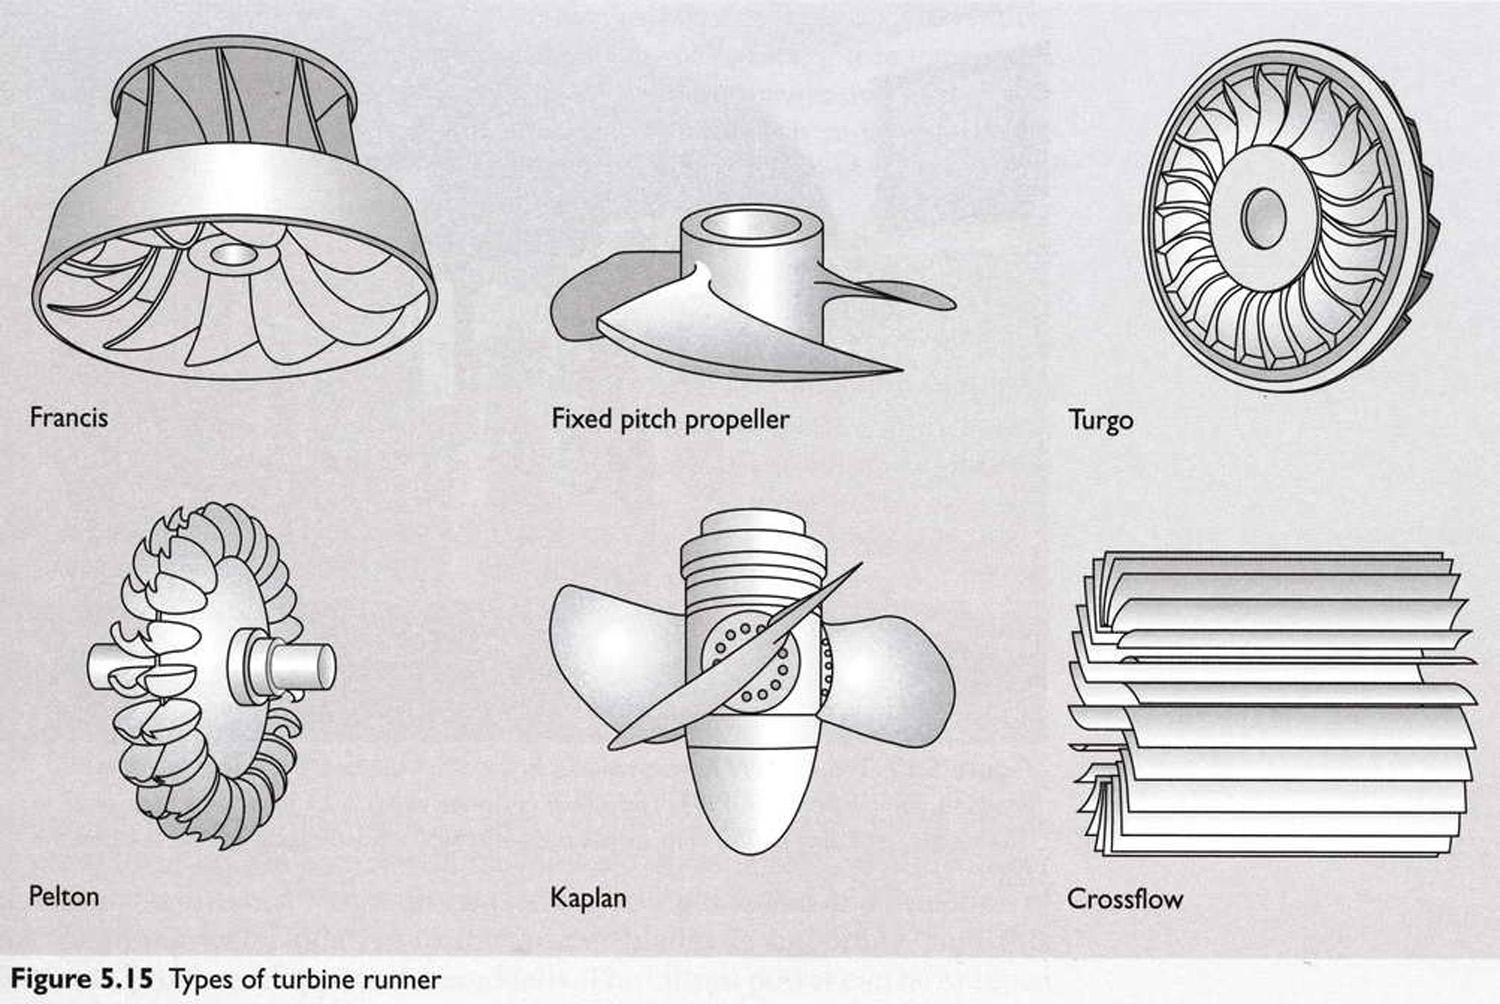
\includegraphics[width=0.9\textwidth]{./pictures/turbines.png}
	\end{frame}
\begin{frame}
		\begin{center}
		\Huge	Thanks for your attention.
\end{center}
\end{frame}

% Alternatively, special title page command to get a different background
% \ntnutitlepage


\end{document}
